\documentclass[a4paper, 25pt]{article}
\usepackage[utf8]{inputenc}
\usepackage[english,russian]{babel}
\usepackage{amsmath,amssymb,amsfonts,textcomp,latexsym,amsopn}
\usepackage{cite,enumerate,float,indentfirst}
\usepackage{graphicx,xcolor}
\begin{document}

\begin{flushright}
Кобзарев Алексей, Тескер Константин, Белозёров Михаил, Рыбаков Владислав.
\\
410 группа
\end{flushright}

\begin{center}
\bfseries ОТЧЕТ ПО ПРАКТИКУМУ НА ЭВМ
\end{center}

\section{Постановка задачи}

Была поставлена задача написания программы проводящей расчёт течения в каверне разностной схемой. 
Система уравнений, описывающая нестационарное движение баротропного газа в область $\Omega$ размерности два, выглядит следующим образом

\begin{equation}
% \frac{\partial p}{\partial t} + div(\rhou) = 0,\\
 \rho[\frac{\partial u}{\partial t} + (u, \bigtriangledown)u]  + \bigtriangledown p = Lu + \rho f, ~~
 p = p (\rho).
\end{equation}
где $L$ есть линейный симметричный положительно определенный оператор.

В данном случае рассматривалась схема описывающая поведение плотности и скорости газа в каверне.

\section{Гладкое решение}

Для проверки правильности формул и работы программы были проведены тесты на гладком решении. В качестве гладкого решения для плотности и скорости были выбраны следующие функции:

$$u1 = sin (2x) \cdot sin (2y) \cdot e^t$$
$$u2 = sin (2x) \cdot sin (2y) \cdot e^{-t}$$
$$\rho = (cos (2x) + 1.5) \cdot (sin (2y) + 1.5) \cdot e^t$$


Для проверки решения далее приведены значения норм разности решения и действительного значения для различных сеток, а также таблица времени работы программы.

\begin{center}
 $C$-норма ошибки для $g: \quad p_{\rho}=10.000, \mu = 0.010 $
\begin{tabular}{|p{0.6in}|p{0.7in}|p{0.7in}|p{0.7in}|p{0.7in}|} \hline
$\tau\setminus h$ & $0.05$ & 0.025& 0.0125 & 0.00625 \\ \hline
$0.00010$ & $5.713e-03$ &$1.271e-02$ &$1.522e-02$ &$1.564e-02$  \\ \hline
$0.00005$ & $3.398e-03$ &$1.072e-03$ &$1.418e-02$ &$1.467e-02$  \\ \hline
$0.00003$ & $2.162e-03$ &$8.986e-03$ &$1.176e-02$ &$1.158e-02$  \\ \hline
$0.00001$ & $1.784e-03$ &$5.674e-03$ &$1.022e-02$ &$7.961e-03$  \\ \hline
\end{tabular}\\[20pt]
\end{center}

\begin{center}
 $L_2$-норма ошибки для $g: \quad p_{\rho}=10.000, \mu = 0.010 $
\begin{tabular}{|p{0.6in}|p{0.7in}|p{0.7in}|p{0.7in}|p{0.7in}|} \hline
$\tau\setminus h$ & $0.05$ & 0.025& 0.0125 & 0.00625 \\ \hline
$0.00010$ & $2.886e-03$ &$3.516e-03$ &$3.660e-03$ &$3.628e-03$  \\ \hline
$0.00005$ & $2.165e-03$ &$2.221e-03$ &$1.984e-03$ &$2.094e-03$  \\ \hline
$0.00003$ & $1.278e-03$ &$1.356e-03$ &$1.012e-03$ &$1.131e-03$  \\ \hline
$0.00001$ & $8.456e-04$ &$8.811e-04$ &$6.641e-04$ &$5.612e-04$  \\ \hline
\end{tabular}\\[20pt]
\end{center}

\begin{center}
$C$-норма ошибки для $v1: \quad p_{\rho}=10.000, \mu = 0.010 $
\begin{tabular}{|p{0.6in}|p{0.7in}|p{0.7in}|p{0.7in}|p{0.7in}|} \hline
$\tau\setminus h$ & $0.05$ & 0.025& 0.0125 & 0.00625 \\ \hline
$0.00010$ & $1.243e-02$ &$1.909e-02$ &$3.166e-02$ &$5.695e-02$  \\ \hline
$0.00005$ & $1.120e-02$ &$1.441e-02$ &$2.012e-02$ &$3.214e-02$  \\ \hline
$0.00003$ & $8.829e-03$ &$9.822e-03$ &$1.313e-02$ &$2.101e-02$  \\ \hline
$0.00001$ & $8.942e-03$ &$5.172e-03$ &$1.065e-02$ &$1.239e-02$  \\ \hline
\end{tabular}\\[20pt]
\end{center}

\begin{center}
 $L_2$-норма ошибки для $v1: \quad p_{\rho}=10.000, \mu = 0.010 $
\begin{tabular}{|p{0.6in}|p{0.7in}|p{0.7in}|p{0.7in}|p{0.7in}|} \hline
$\tau\setminus h$ & $0.05$ & 0.025& 0.0125 & 0.00625 \\ \hline
$0.00010$ & $4.312e-03$ &$1.944e-03$ &$1.580e-03$ &$1.494e-03$  \\ \hline
$0.00005$ & $2.781e-03$ &$1.583e-03$ &$1.181e-03$ &$1.291e-03$  \\ \hline
$0.00003$ & $1.661e-03$ &$7.163e-04$ &$7.120e-04$ &$8.134e-04$  \\ \hline
$0.00001$ & $7.127e-04$ &$5.041e-04$ &$4.981e-04$ &$5.828e-04$  \\ \hline
\end{tabular}\\[20pt]
\end{center}

\begin{center}
 $C$-норма ошибки для $;v2: \quad p_{\rho}=10.000, \mu = 0.010 $
\begin{tabular}{|p{0.6in}|p{0.7in}|p{0.7in}|p{0.7in}|p{0.7in}|} \hline
$\tau\setminus h$ & $0.05$ & 0.025& 0.0125 & 0.00625 \\ \hline
$0.00010$ & $8.334e-03$ &$1.335e-02$ &$2.638e-02$ &$5.207e-02$  \\ \hline
$0.00005$ & $7.124e-03$ &$1.002e-02$ &$1.932e-02$ &$2.321e-02$  \\ \hline
$0.00003$ & $3.212e-03$ &$7.125e-03$ &$1.132e-02$ &$1.781e-02$  \\ \hline
$0.00001$ & $2.018e-03$ &$4.334e-03$ &$6.212e-03$ &$1.183e-02$  \\ \hline
\end{tabular}\\[20pt]
\end{center}

\begin{center}
$L_2$-норма ошибки для $v2: \quad p_{\rho}=10.000, \mu = 0.010  $
\begin{tabular}{|p{0.6in}|p{0.7in}|p{0.7in}|p{0.7in}|p{0.7in}|} \hline
$\tau\setminus h$ & $0.05$ & 0.025& 0.0125 & 0.00625 \\ \hline
$0.00010$ & $5.452e-03$ &$4.130e-03$ &$3.862e-03$ &$4.539e-03$  \\ \hline
$0.00005$ & $3.123e-03$ &$2.722e-03$ &$2.257e-03$ &$2.711e-03$  \\ \hline
$0.00003$ & $2.320e-03$ &$1.938e-03$ &$1.201e-03$ &$2.121e-03$  \\ \hline
$0.00001$ & $1.491e-03$ &$1.129e-03$ &$7.620e-04$ &$1.240e-03$  \\ \hline
\end{tabular}\\[20pt]
\end{center}

\begin{center}
Время, $p_{\rho}=10.000, \mu = 0.010  $
\begin{tabular}{|p{0.6in}|p{0.7in}|p{0.7in}|p{0.7in}|p{0.7in}|} \hline
$\tau\setminus h$ & $0.05$ & 0.025& 0.0125 & 0.00625 \\ \hline
$0.00010$ & $8.603e-03$ &$2.935e-02$ &$1.295e-01$ &$7.603e-01$  \\ \hline
$0.00005$ & $1.550e-02$ &$5.310e-02$ &$2.467e-01$ &$1.341e+00$  \\ \hline
$0.00003$ & $3.005e-02$ &$9.889e-02$ &$4.552e-01$ &$2.554e+00$  \\ \hline
$0.00001$ & $5.630e-02$ &$1.962e-01$ &$8.307e-01$ &$4.615e+00$  \\ \hline
\end{tabular}\\[20pt]
\end{center}


Результаты свидетельствуют о том, что программа реализована верно и имеет место сходимость решения к действительному значению плотности и скорости.
\newpage

\section {Численные эксперименты}

Были проведены численные эксперименты, моделирующие реальных условий.
Блыли реализованы четыре версии программы описываще различные по форме каверны.
Начальные условия были установлены следующие:\\
Белозёров Михаил
\begin {itemize}
\item Область $\Omega = \Omega_{02} \cup \Omega_{12} \cup \Omega_{22} \cup \Omega{11} \cup \Omega{21} \cup \Omega{10} \cup \Omega_{20}$
  \item $u_1|_{\Gamma_{02}^{x-}} = \omega$
  \item $\frac{{\partial}u_2}{{\partial}y}|_{\Gamma_{10}^{y-}\cup\Gamma_{20}^{y-}} = 0$
\end   {itemize}
Кобзарев Алексей
\begin {itemize}
\item Область $\Omega = \Omega_{00} \cup \Omega_{10} \cup \Omega_{01} \cup \Omega{11} \\ \Gamma^{x+}_{00}$
  \item $u_2|_{\Gamma_{00}^{Y-}} = \omega$
  \item $\frac{{\partial}u_2}{{\partial}y}|_{\Gamma_{10}^{y-}} = 0$
\end   {itemize}


Для выяснения корректности проведенных экспериментов была написана дополнительная программа, визуализирующая результаты проделанных экспериментов. Было замечено, что при увеличении временного парметра решение стабилизируется и результаты для каждой из задач выглядят следующим образом: \\
Белозёров Михаил:
\begin{figure}[h!]
\center{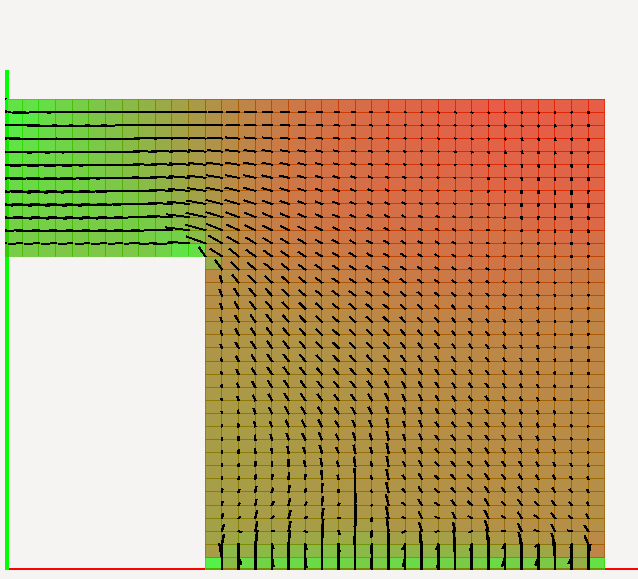
\includegraphics[width=0.7\linewidth]{screen_belozerov.jpg}}
\end{figure}
\\
\newpage
Кобзарев Алексей:
\begin{figure}[h!]
\center{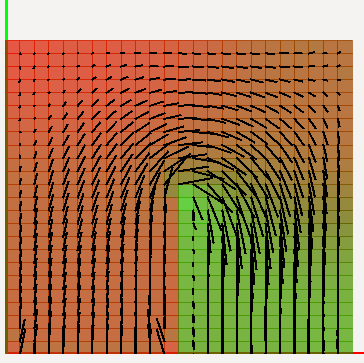
\includegraphics[width=0.7\linewidth]{screen_kobzarev.png}}
\end{figure}
\\
\\
Плотность газа характеризуется цветом ячейки. От зелёного к красному по возрастанию значения плотности. Черные палочки -- вектора скорости.

\newpage
\section{Сходимость и собственные функции}
Были проведены эксперименыты по скорости сходимости для изначального решения. Результаты приведены ниже.

Для матрицы были вычислено время установления стационарного решения и время восстановления его после возмущения. Были вычислены собственные значения
и их собственные вектора оператора линеаризации, а также проведены численные эксперименты, использующие полученные возмущения функций плотности и 
скорости. Ниже приведены результаты (возмущение считалось только для действительных собственных значений):
\begin{itemize}
 \item $-3.015234e-01 \pm 1.792826e-01$: время = 2085
 \item $-3.168194e-01 \pm 1.331842e-01$: время = 352
 \item $-1.652393e-01 \pm 1.205335e-01$: время = 293
 \item $-2.348801e-01$: время = 187
 \item $-1.784789e-01$: время = 315
 \item $-1.898415e-01$: время = 347 
\end{itemize}
Отсюда можно сделать вывод, что чем меньше собственное значение, тем быстрее оно сходится при малых возмущениях.
\section{Описание реализации}
Программа реализована на языке С, опираясь на исходный код выданной программы и используя пакет laspack.
Для реализации были созданы масивы инндексирующие связь плотности и скорости. Массивы назваются left bottom v - индекс скорости стоящей на пол узла ниже и пол узла левее плотности.
left h index -  индекс плотности на полл узла правее и пол узла выше узла скорости
left top h index -  индекс плотности на полл узла левее и пол узла выше узла скорости

nак же для облегчения работы с индексами были ввеедены два массива hv map и vh map jтвечающие за соответствие узлов скорости и плотности.

Для реализации заполнения сетки и начальных данныхбыли написаны функции set arrays for H, reset H index, setka for v.\\
Схема решения притерпела небольшие изменения. Вместо одного вычисления матрицы размерности $DIM_H + 2 * DIM_V$ теперь используется две матрицы размерности $DIM_H$ для плотности  и размерности $2 * DIM_V$ для скорости. На каждом шаге по времени происходит сначала вычисление плотности по данным с предыдущего шага. Затем просиходит вычисление скорости по плотности с новго шага и значений сокрости с предыдущего шага. 

Для вычисления индексов для узла были добавлены функции fill for H и fill for v.
Для заполенения матриц использвуются функции cases H и case 0 V, case 1 8 V. Так как скорости на границах полагаются известными то разбирать случаи граничных узлов не имеет смысла, для них написан общий случай выставления диагонального элемента значение 1 и правой части с действительным значением скорости в этом узле.

\section{Заключение}
В результате проведенных экспериментов было установлено, что схема даёт правдивые результаты и может быть использована для расчётов реальных моделей течения газов. 
\end{document}
